\documentclass[11pt]{article}
\usepackage[includeheadfoot, top=1.0in, bottom=1.0in, hmargin=1.0in]{geometry}
\usepackage[utf8]{inputenc}
\usepackage{fancyhdr}
\pagestyle{fancy}
\usepackage{setspace}
\usepackage{tabularx}
\usepackage{xcolor}
\usepackage{cancel}
\usepackage{amsmath,amsfonts}
\usepackage{graphicx}
\usepackage{siunitx}
\usepackage{amssymb}

\usepackage[hyphens]{url}
\usepackage{hyperref}
\usepackage{enumitem}

\lhead{Astronomy Lab II}
\rhead{Spring 2022}
\lfoot{Mead}
\rfoot{Mon 6-9pm}
\cfoot{\thepage}

\begin{document}

\begin{center}
\huge{Lab 9: Hubble's Law}\\ \medskip \Large{April 4, 2022}
\end{center}

\section{Introduction: The Expanding Universe}
In 1929, Edwin Hubble made a discovery that would change the course of astronomy forever. While poring over data on the distances and velocities of faraway galaxies, Hubble noticed two things: one, that almost all galaxies are systematically moving \emph{away} from us; and two, that galaxies that are \emph{further} away from us are moving away \emph{faster}. From these observations, Hubble drew a simple -- but groundbreaking -- conclusion: \textbf{space itself is expanding}.  

\begin{figure}[h!]
    \centering
    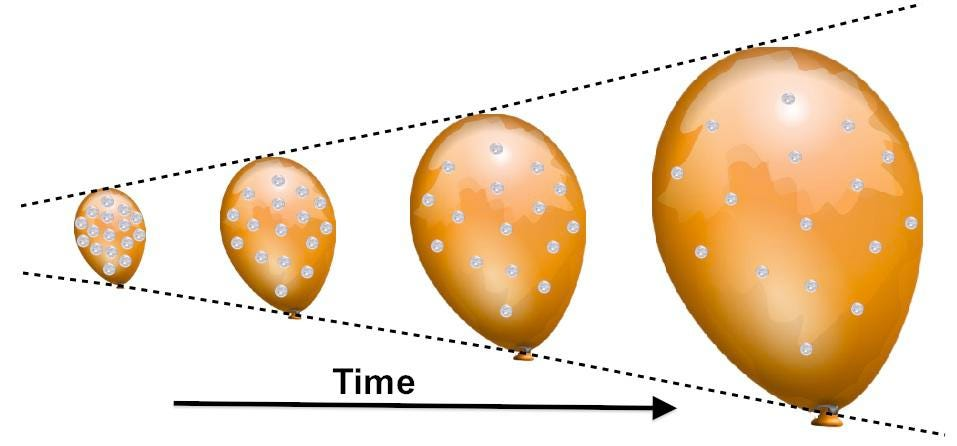
\includegraphics[width=0.6\textwidth]{Images/expanding balloon.jpg}
    \caption{An expanding balloon analogizing the expanding Universe.}
    \label{fig:balloon}
\end{figure}
\noindent
Consider Figure \ref{fig:balloon}, showing a balloon covered in stickers. While these stickers themselves aren't moving, the expansion of the balloon pushes them apart. Now, imagine that these stickers are galaxies and that the balloon is the expanding Universe. While a galaxy may not have its own intrinsic velocity, it'll still appear to move away from us due to the expansion of space itself. Therefore, distant galaxies acquire a \emph{redshift} due solely to cosmological expansion.

\medskip \noindent
If the Universe is \emph{expanding}, then it must have a finite age; at some time in the distant past, the Universe was just a point. Hubble's discovery thus revolutionized the field of cosmology -- the study of the history and composition of the Universe -- paving the way for theories of the Big Bang, of galaxy formation and evolution, of the birth of the first stars, and so much more.

\medskip \noindent
In today's lab, we will trace how our understanding of Hubble's discovery has evolved over time. We will also learn how to measure the expansion rate of the Universe via the \emph{cosmic distance ladder}. This lab should leave you with a deeper understanding of \emph{Hubble's law}, which forms the foundation of modern cosmology.

\section{Hubble Trouble: Finding the Expansion Rate of the Universe}

Mathematically, the expansion of the Universe is encoded in \textbf{Hubble's Law},
\begin{equation} \label{eq:hubble}
    v = H_0 D,
\end{equation}
which states that the velocity, $v$, of an object moving due to the expansion of space is related to the object's distance, $D$, via some constant, $H_0$. $H_0$, or the \textbf{Hubble constant}, therefore tells us \emph{how fast} the Universe is expanding. According to equation \ref{eq:hubble}, we can find this expansion rate by making a plot of velocity vs. distance (for many distant astronomical objects) and measuring the \emph{slope} of the line that best fits the data. In this section, we'll see how this works out in practice.

%This paper will be useful for writing this section: \url{https://arxiv.org/pdf/2002.02439.pdf}% 

\subsection{Retracing Hubble's steps}

Let's travel back in time to 1929, when Hubble was working out his theory of the expanding Universe. Given that, just a few years prior, Hubble had shown that other galaxies were in fact \emph{outside of} the Milky Way, we can assume that telescope data in the 1920s wasn't fantastic. 

\medskip \noindent
On CourseWorks (in the Lab 9 folder under ``Files''), open the spreadsheet titled ``hubble.xlsx''; the first tab (labeled ``1929'') shows Hubble's original data for 24 galaxies. Note that the velocity is labeled ``recession velocity'' -- this means that we're looking only at motions towards or away from us.  \textbf{Be sure to include the appropriate graphs in your lab write-up.}

\begin{enumerate}
    \item Make a scatter plot of Hubble's data, putting recession velocity (in km/s) on the vertical axis and distance (in Mpc) on the horizontal axis. For reference, 1 Mpc (``megaparsec'') is about 3 million light years, or about $3 \times 10^{19}$ kilometers.
    
    \item On the same figure, plot the line that best fits the data. In Google Sheets, you can do this by going to the ``Customize'' tab under the chart editor, clicking ``Series,'' and then checking the box labeled ``Trendline.'' 
        \begin{enumerate}
            \item Hubble's law predicts a linear trend between recession velocity and distance. How well does your trend line fit the data? Are you convinced that there's actually a linear trend in the data? 
            
            \item Why doesn't the line perfectly fit the data? That is, what are some sources of error or uncertainty that could be causing deviation from the predicted linear model?
            
            \item Does your line pass through the origin (i.e., does your line pass through the point of zero velocity and zero distance)? Do you expect the line to pass through the origin? (Hint: think about Equation \ref{eq:hubble})
            
            \item If your line doesn't pass through the origin, \emph{why} doesn't it? 
        \end{enumerate}
    
    \item Slightly below the check box for ``Trendline,'' there's a drop-down menu for ``Label;'' set this to ``Use Equation,'' and enable the check-box labeled ``Show $R^2$'' below it.
        \begin{enumerate}
            \item For this best-fit line, what should be the \emph{units} of the slope? (Hint: remember that slope is ``rise over run,'' or the vertical change divided by the horizontal change)
            
            \item The equation of the best-fit line should be of the form $m \times x + b$, where $m$ is the slope and $b$ is the y-intercept. What is the slope of your best-fit line (remember to add units)? Congrats -- you've just measured the Hubble constant!
            
            \item What value do you get for $R^2$? $R^2$ is a measure of how good the line fits the data, with $R^2 = 1$ being a perfect fit. Would you characterize this linear model as a ``good'' fit?
        \end{enumerate}
        
    \item Since the Hubble constant tells us how fast the Universe is (and has been) expanding, it also tells us how \emph{old} the Universe is. We can obtain a rough estimate for the age of the Universe by taking the reciprocal of the Hubble constant, or $1/H_0$.
    \begin{enumerate}
        \item The Hubble constant has weird units, so we'll first have to do some unit conversion. $1 \rm \, \frac{km/s}{Mpc} = 1.02 \times 10^{-12} \frac{1}{year}$. Use this to convert your measurement of $H_0$ to units of $\frac{1}{\rm year}$.
        
        \item Now, compute $1/H_0$ to obtain the age of the Universe in years. Does your answer make sense?
        
        \item Using radiometric dating of rocks, geologists have determined the age of the Earth to be about $4.5 \times 10^9$ years old. How does this compare to your estimate of the age of the Universe? Does this make sense?
    \end{enumerate}
\end{enumerate}

\subsection{Improving on our results}
% Data taken from Freedman et al. 2001, "Final Results from the Hubble Space Telescope Key Project to Measure the Hubble Constant"

A lot has changed since 1929. With fancy new space telescopes, we can now see significantly deeper into space and take measurements with significantly higher precision. Let's compare Hubble's 1929 data to some more recent data.

\medskip \noindent
On the ``hubble.csv'' spreadsheet, go to the second tab, labeled ``Key Cepheids.'' This sheet contains measurements of 24 Cepheid variable stars taken by the Hubble Space Telescope between 2000 and 2001. Cepheids possess special properties that make them good distance indicators (which we'll cover in \S\ref{sec:cepheids}); if we can find a Cepheid in a distant galaxy, then we can obtain the distance to that galaxy. Edwin Hubble's original paper actually used Cepheid data as well, but note the difference in the distance range between the old data set and the new one: while the largest distance in the 1929 paper is 2.0 Mpc, these 2001 measurements go all the way up to 21.98 Mpc.

\begin{enumerate}
    \item For the ``Key Cepheids'' data set, again plot recession velocity on the vertical axis and distance on the horizontal axis. As before, overlay the line of best fit and obtain the equation for the line.
    
    \item What is the value of $R^2$ when fitting a line to this data set? Is this fit better or worse than the fit to the 1929 data set? Why do you think this is the case?
    
    \item What value of $H_0$ do you measure for this data set? How does this compare to the $H_0$ you measured for the 1929 data set? 
    
    \item Without doing any math, do you expect the age of the Universe inferred from the 1929 data to be higher or lower than that inferred from the 2001 Hubble Telescope data? Explain intuitively why this is the case, without appealing to any math (remember: a higher $H_0$ means that the Universe is expanding \emph{faster})
    
    \item Use your new value of $H_0$ to recompute the age of the Universe (in years). Was your intuition from the previous question correct?
    
    \item Compare your new value for the Universe's age to the Earth's age ($4.5 \times 10^9$ years). Does this make sense? 
    
    \item Now, plot the 1929 data and the 2001 Cepheid data on the same graph by highlighting columns B, C, and D on the sheet labeled ``Combined". 
    \begin{enumerate}
        \item Briefly describe what the plot looks like.
        
        \item Edwin Hubble's original data and the Hubble Space Telescope's data should look noticeably different, despite the fact that they're both measurements of Cepheid variable stars in the nearby Universe. What are two possible reasons for the differences in these two data sets?
        
        \item Could your two values for $H_0$ still be ``consistent,'' even if they're numerically different? Why or why not? Think about the uncertainty or error associated with any scientific measurement. 
        
        \item The galaxy NGC 7331 actually shows up in both data sets. What are the distance and recession velocity of this galaxy in each data set? You should notice that something is weird -- how do you justify this?
    
    \end{enumerate}
\end{enumerate}
\noindent
More recently, it's become popular to measure the Hubble constant using \emph{Type Ia supernovae} -- the explosions of white dwarf stars -- since they can provide reliable distance measurements to very faraway galaxies. The third tab in the ``hubble.csv'' spreadsheet (labeled ``Key SNIa'') contains distance and velocity measurements of Type Ia supernovae taken by the Hubble Space Telescope between 2000 and 2001 (during the same survey that produced the ``Key Cepheids'' data set). 

\begin{enumerate}[resume]
    \item What is the difference between the largest distance measured in the ``Key SNIa'' data set and the largest distance measured in the ``Key Cepheids'' data set?
    
    \item Plot the supernova data as usual and find the associated value for the Hubble constant. How does this $H_0$ measurement compare to the other two values you've found?
    
    \item Compare the $R^2$ value of the linear fit to this data set to the $R^2$ values from the other two data sets. As we take measurements out to larger and larger distances, does our data agree more or less with Hubble's law? Why might this be the case? (stay tuned for Section 3)
\end{enumerate}


\subsection{The limits of Hubble's law}

In the late 1990s, there was fierce competition between the Supernova Cosmology Project (lead by Saul Perlmutter at Berkeley) and the High-Z Supernova Search Team (led by Brian Schmidt at Harvard and Adam Riess at the Space Telescope Science Institute) to measure the most distant Type Ia supernovae possible, and thus to produce the highest-quality measurements of the Hubble constant. Both teams stumbled upon some strange results.

\begin{figure}[h!]
    \centering
    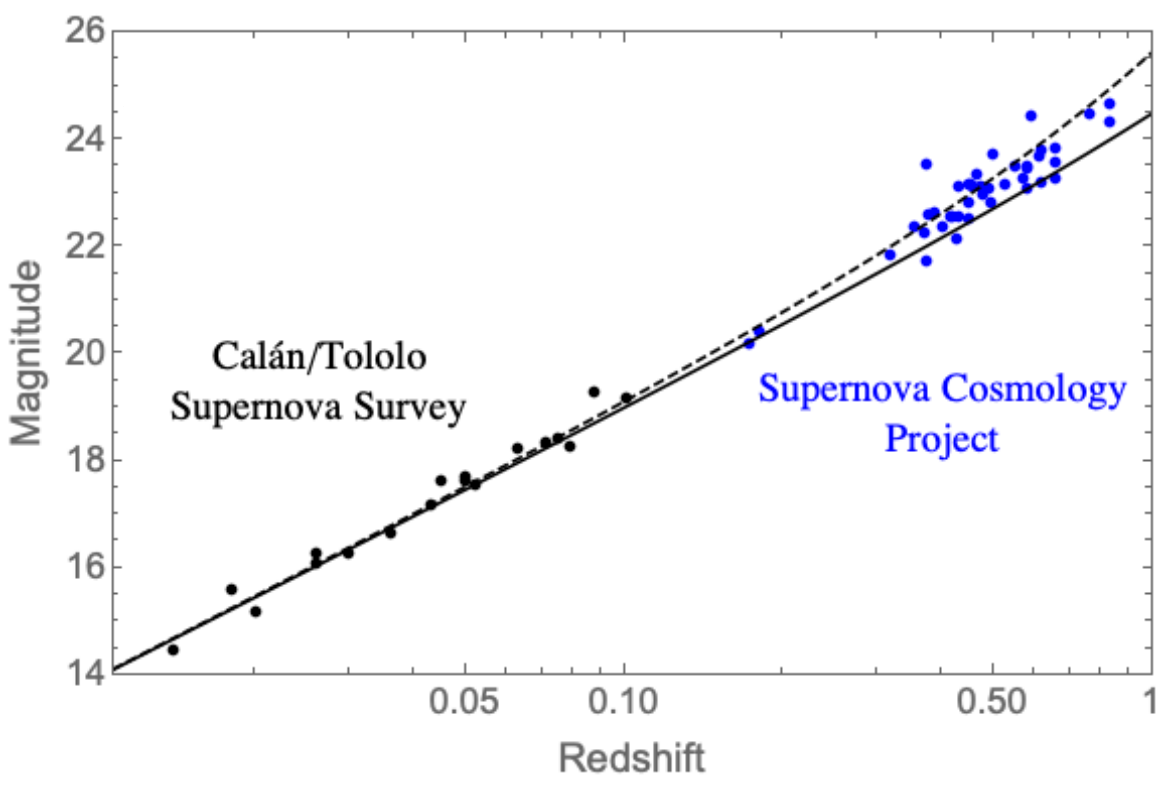
\includegraphics[width=0.6\textwidth]{Images/acceleration2.PNG}
    \caption{Data from the Supernova Cosmology Project showing deviation from Hubble's law at very large distances.}
    \label{fig:acceleration}
\end{figure}
\medskip \noindent
Figure \ref{fig:acceleration} shows the Supernova Cosmology Project's data alongside older supernova data taken at shorter distances; here, magnitude is a proxy for distance and redshift is a proxy for velocity, so the axes are actually \emph{flipped} compared to what we've been plotting. 
\begin{enumerate}
    \item Describe the trend in Figure \ref{fig:acceleration} at large distances (i.e., at large magnitude and redshift). Does the data still follow the linear trend predicted by Hubble's law?
    
    \item According to Hubble's law, objects that are more distant from us are receding from us faster, and thus the light emitted by more distant objects will be more redshifted. Light from more distant objects also takes longer to reach us, so more distant objects appear to be younger, or to have existed earlier in the Universe. In this sense, how can we use redshift as a proxy for cosmic time?   
    
    \item In Figure \ref{fig:acceleration}, a higher redshift corresponds to an object that existed earlier in the Universe; therefore, moving from high redshift to low redshift shows a progression from past to present. Given this, how has the Hubble constant (the slope of the best-fit line) evolved over time? Remember that the axes here are \emph{reversed} with respect to our previous plots!
\end{enumerate}

\noindent
This is a tricky plot to analyze, but you should have concluded that $H_0$ is getting \emph{larger} over time -- that is, the Universe's expansion is \emph{accelerating}. While this discovery earned Perlmutter, Schmidt, and Riess the 2011 Nobel Prize in Physics, we still don't actually know \emph{why} the Universe is accelerating. We therefore call the mysterious force accelerating the Universe \textbf{dark energy}.  

\begin{figure}[h!]
    \centering
    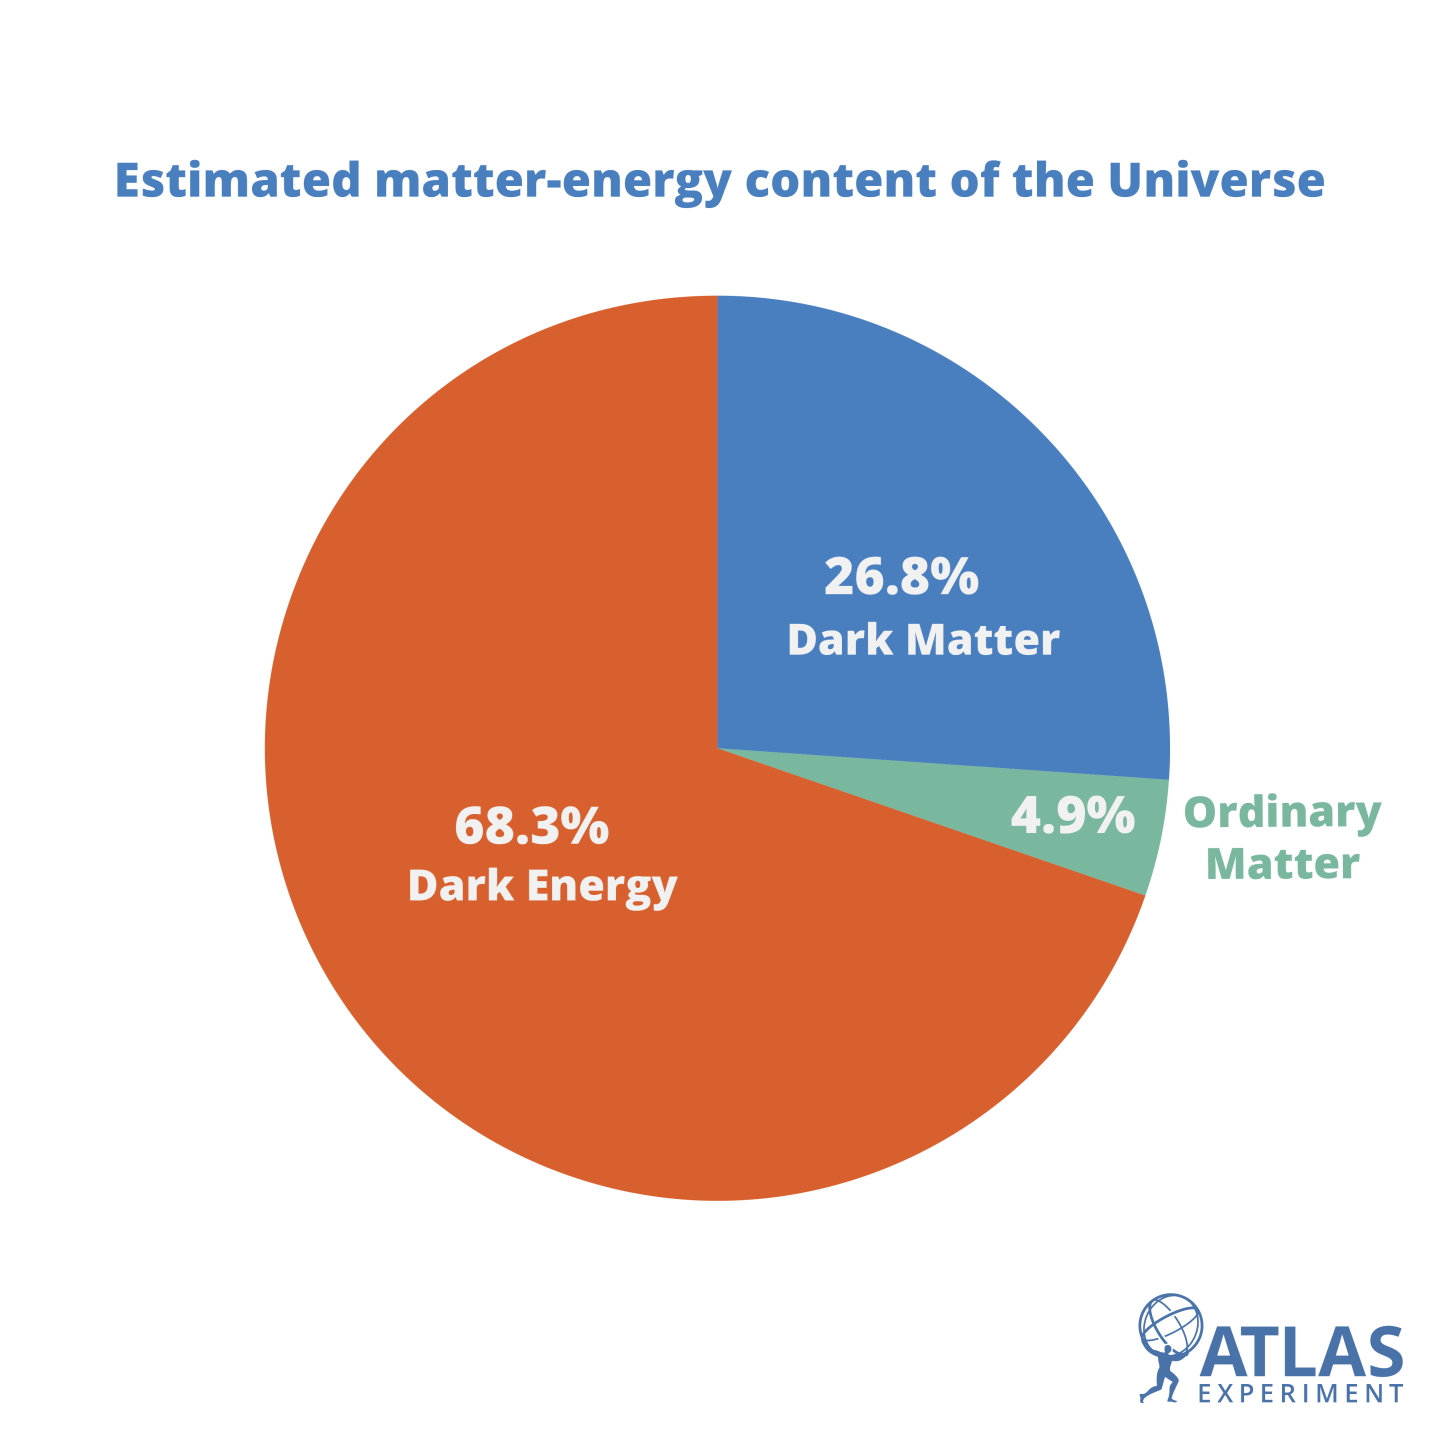
\includegraphics[width=0.6\textwidth]{Images/dark energy.png}
    \caption{Energy content of the Universe.}
    \label{fig:energy}
\end{figure}
\medskip \noindent
It turns out that dark energy dominates the energy content of the Universe (see Figure \ref{fig:energy}). Matter and dark energy are locked in an endless struggle to control the fate of the Universe: while matter wants to pull things together and slow the Universe's expansion, dark energy wants to push the Universe apart.
\begin{enumerate}[resume]
    \item Cosmologists believe that dark energy will forever remain dominant over matter. If this is the case, what will be the ultimate fate of the Universe?
    
    \item If, somehow, matter were to become dominant over dark energy, how would this affect the ultimate fate of the Universe?
\end{enumerate}


\section{A Stairway to Heaven: The Cosmic Distance Ladder}

In the previous section, you should have found that Hubble's original data had a significant amount of scatter, thus yielding a value for $H_0$ that's very different from what we'd obtain with more recent data. One major source of error in Hubble's data was that the galaxies he studied were \emph{too close} to us; in the local Universe, gravitational interactions between galaxies compete against the expansion of space, causing deviations from Hubble's law. Therefore, to ensure that our measured velocities are due solely to the Universe's expansion, we must look at very distant galaxies that are free from the gravitational influence of the Milky Way and its neighbors. We say that these distant galaxies move purely with the ``Hubble flow.''

\medskip \noindent
Unfortunately, measuring large distances in astronomy is \emph{difficult}. But, with a technique known as the \textbf{distance ladder}, we can use measurements of shorter distances to gradually build up to measurements of huge, cosmological distances (which we can then plug into Hubble's law). For instance, we can use \emph{parallax} to find the distances to nearby Cepheid variable stars; we can use nearby Cepheid variables to calibrate the Cepheid \emph{period-luminosity} relationship, giving us the distances to farther Cepheids; we can use the distances of Cepheids in faraway galaxies to calibrate the light curves of distant supernovae; and we can use these supernova light curves to estimate the Hubble constant.

\medskip \noindent
In this section, you will learn about a few key techniques that form the ``rungs'' of our cosmic distance ladder.

\subsection{Parallax}

\textbf{Parallax} is the change in the \textsl{apparent position} of an object when viewing it from \textsl{two different lines of sight} (i.e., perspectives). An illustration of this phenomenon is shown in Fig \ref{fig:parallax_example} (left), where the object covers the distant blue square when viewed from ``Viewpoint A" but instead covers the distant red square when viewed from ``Viewpoint B".

\begin{figure}[h!]
    \centering
    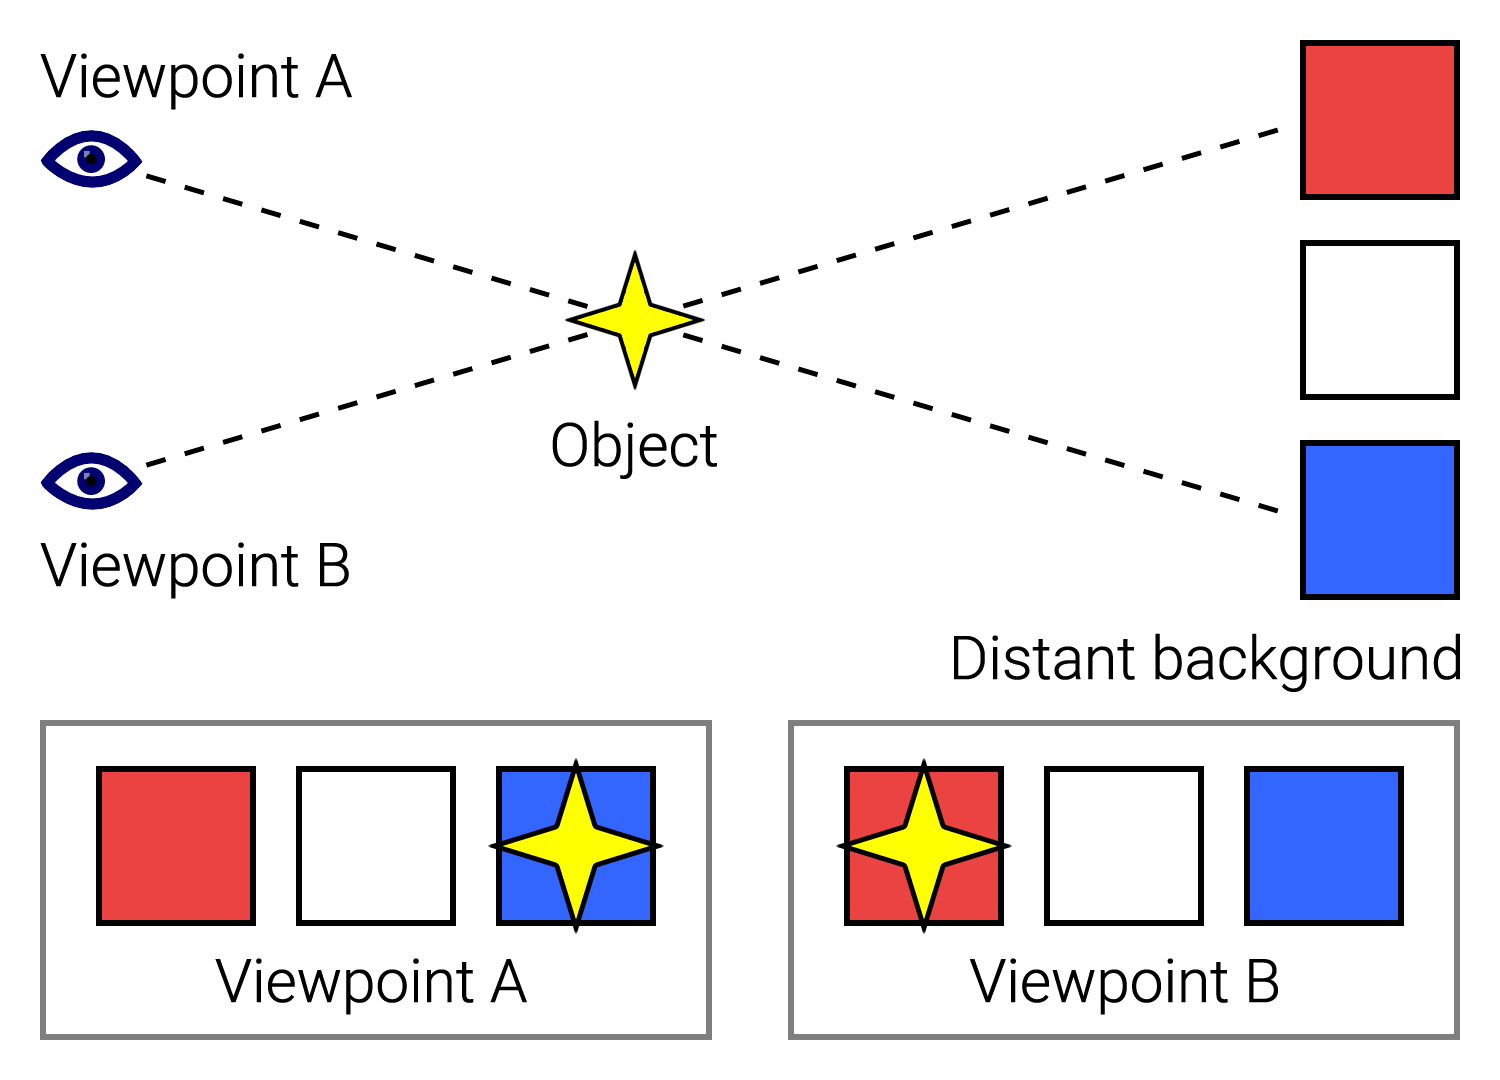
\includegraphics[width=0.5\textwidth]{Images/Parallax_Example.png}
    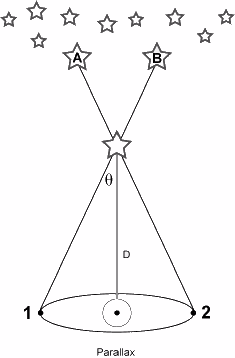
\includegraphics[width=0.3\textwidth]{Images/parallax.png}
    \caption{(\textsl{Left}) A simplified illustration of the parallax of an object against a distant background due to a perspective shift. (Credit: \href{https://en.wikipedia.org/wiki/Parallax\#/media/File:Parallax_Example.png}{Wikipedia} \href{https://creativecommons.org/licenses/by-sa/3.0/}{CC BY-SA 3.0}). (\textsl{Right}) Parallax in the context of astronomy. Points 1 and 2 indicate positions of the Earth 6 months apart, with the circled dot representing the Sun. Parallax in the context of astronomy. Points 1 and 2 indicate positions of the Earth 6 months apart, with the circled dot representing the Sun.}
    \label{fig:parallax_example}
\end{figure}

\noindent
You can try this out yourself. Extend your arm and put your thumb up. Close one of your eyes and move your thumb around until you cover something in the (distant) background. Without moving your thumb, switch your open eye and notice how the \textsl{apparent position} of your thumb has changed relative to the background. Bring your thumb closer and do the same. Did the apparent change in your thumb's position become smaller or larger? 

% \begin{figure}[h!]
%     \centering
%     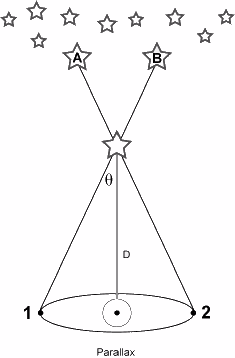
\includegraphics[width=0.3\textwidth]{Images/parallax.png}
%     \caption{Parallax in the context of astronomy. Points 1 and 2 indicate positions of the Earth 6 months apart, with the circled dot representing the Sun.}
%     \label{fig:parallax_star}
% \end{figure}
\medskip \noindent
It turns out that this geometric phenomenon is a powerful tool for measuring the distance to relatively nearby stars. Figure \ref{fig:parallax_example} (right) shows how parallax works in the context of astronomy. When viewed from point 1, the star at the tip of the triangle will look like it as at position B, while if it is viewed from point 2 it will look like it is at position A. Let's define $D$ to be the distance between the Sun and the other star, $B$ to be the ``baseline'' (the distance between point 1 and point 2), and $\theta$ to be the ``parallax angle'' (defined as \textsl{half} the angle separating A and B of the object). Notice that, in Figure \ref{fig:parallax_example} (right), the star, the Sun, and point 1 create a right triangle. Since $\tan\theta = \frac{\mathrm{opposite}}{\mathrm{adjacent}} = \frac{B/2}{D}$, you can obtain an expression for the distance, $D$, as 
\begin{equation} \label{eq:parallax}
    D = \frac{B/2}{\tan\theta} \approx \boxed{\frac{B/2}{\theta}},
\end{equation}
where we replaced $\tan\theta$ with $\theta$, since these angles are typically quite small (you can check for yourself that $\tan\theta$ is very close to $\theta$ for very small $\theta$).

\medskip \noindent
Using Equation \ref{eq:parallax}, \textbf{answer the following questions in your lab write-up:}

\begin{enumerate}
    \item For an object at a fixed distance, how does $\theta$ change as you increase $B$? 
    
    \item For a fixed $B$, how does $\theta$ change as $D$ increases?
\end{enumerate}

\subsubsection{Using parallax to measure the length of your arm}

Using the expression you derived for obtaining the distance $D$ from the baseline $B$ and the parallax angle $\theta$, let's try to measure the length of your arm via parallax. For this activity we'll use an instrument called a \emph{sextant} to measure angles. Sextants have historically been very useful tools for figuring out your location based on the positions of astronomical objects (i.e., celestial navigation). Sextants are usually used to measure the vertical angle of an astronomical source from the horizon, but we'll be using it to measure horizontal angles. 

\begin{enumerate}[label=Step \arabic*:]
    \item Extend your arm and put your thumb up.
    
    \item With one eye open, align one edge of your thumb with some relatively distant object in the background. Make sure you remember this spot since you'll be measuring the angle relative to this point.
    
    \item \textsl{Without moving your thumb or your head}, switch your open eye. Notice the background spot where the same edge of your thumb from the previous step is now located. It should be quite different. Remember this point too as you'll be measuring the angle to this new spot. 
    
    \item Grab the sextant with one hand and squeeze the trigger where the angles are written to re-position it so that it reads $0^\circ$. If you look through the eyepiece (make sure the dark filters are out of the way) you should just see one image.
    
    \item Hold the sextant horizontally so that the back of your right hand is facing the floor, and position yourself so that the image through the eyepiece aligns with the spot from Step 2.
    
    \item \textsl{Without changing the pointing of the sextant}, squeeze the trigger and adjust the mirror until half of the image is now showing the spot from Step 3. 
    
    \item Read off the angle from the sextant and record it in your notebook. This is our parallax angle, $\theta$.
    
    \item Using a ruler or measuring tape, measure the distance between your eyes and record this in your notebook. This is our baseline, $B$.
    
\end{enumerate}

\medskip \noindent
Now, \textbf{complete the following in your lab write-up}:
\begin{enumerate}
\setcounter{enumi}{2}
    \item In order to use the formula for parallax distance that we looked at earlier ($D = \frac{B/2}{\theta}$), we'll first need to convert our angle from \emph{degrees} to \emph{radians}. To do this, multiply the angle you measured with the sextant by $\frac{\pi}{180}$ (or approximately $1.75 \times 10^{-2}$).
    
    \item Using the formula for parallax distance, calculate the length of your arm. Use the angle (in radians) from the previous question for $\theta$ and use the distance between your eyes for $B$.
    
    \item Now, measure the actual length of your arm using a meter stick or tape measure.
    \begin{enumerate}
        \item How well does this measurement agree with the length you computed via parallax?
        
        \item If your two lengths don't agree, why don't they? Think about sources of error and uncertainty in your measurements.
        
        \item To obtain a more accurate length/distance using parallax, is it more important to have an accurate measurement of the distance between your eyes (i.e., the baseline measurement) or to have an accurate measurement of the parallax angle? Why?
    \end{enumerate}
    
    \item Imagine that we apply this same technique to measure the distance to a nearby star.
    \begin{enumerate}
        \item How will the parallax angle change as we move from measuring small distances (i.e., the lengths of our arms) to measuring astronomical distances (i.e., the distances to nearby stars)?
        
        \item What difficulties are introduced in trying to measure parallax distances for objects that are farther and farther away? 
    \end{enumerate}
        
\end{enumerate}



\subsubsection{Parallax in Action: The Gaia Space Observatory}

While the parallax technique can be used to infer the distances of relatively nearby stars in the Universe, parallax measurements at astronomical scales are difficult as they yield extremely small angles. Luckily, for an object at a fixed distance, the parallax angle can be increased by using a \emph{longer baseline}. 

\medskip \noindent
The European Space Agency's \textbf{Gaia space observatory} -- a highly successful ongoing mission measuring the parallax of around 2 \emph{billion} stars in our Galaxy (about 2\% of the galactic stellar population!) -- is able to achieve a baseline equal to the diameter of the Earth's orbit around the Sun (2 AU) by orbiting the Sun alongside the Earth. Take a look at these two short clips: \url{https://youtu.be/m1ZNSPrH0q8?t=168} ;  \url{https://www.youtube.com/watch?v=0-jhyRIupY4} (you can ignore the fact that the parallax ellipses are non-circular in the first video). Gaia is able to precisely measure parallax angles down to $20\;\mu\mathrm{as}$ (micro-arcseconds). An arcsecond (as or $''$) is an astronomical unit of angle, where 1 degree = 60 arcminutes and 1 arcminute = 60 arcseconds. In other words, 1 arcsecond = 1/3600 degrees (see Figure \ref{fig:arcunits}). Since $\mu = 10^{-6}$, Gaia's precision is $20\;\mu\mathrm{as}\approx 5.55\times 10^{-9}\;\mathrm{degrees}$! That's a small angle!!

\begin{figure}
    \centering
    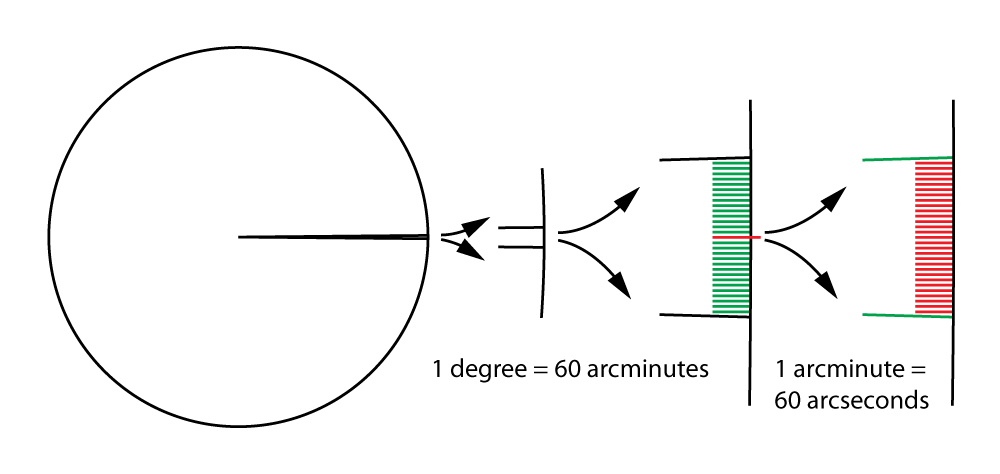
\includegraphics[width=0.5\textwidth]{Images/blog014-image001-degree-arcmin-arcsec.png}
    \caption{1 degree = 3600 arcseconds}
    \label{fig:arcunits}
\end{figure}
\medskip \noindent
\textbf{Answer the following questions in your lab notebook:}

\begin{enumerate}[resume]
    \item Suppose you measure a parallax angle of $1''$ using a baseline of $B=2\;\mathrm{AU}$ ($1\;\mathrm{AU} \approx 1.496\times 10^{11}\;\mathrm{m} \approx 8\;\mathrm{light{-}minutes}$). Using Equation \ref{eq:parallax}, calculate the distance, $D$, to the object. Did you get something close to $206,265\;\mathrm{AU}$? This is how we define the \textbf{parsec} (or pc) -- the distance that produces a \emph{parallax of one (arc)second}.
    
    \item By using parsecs for distance ($D$) and arcseconds for the parallax angle ($\theta$), we can define a simpler relationship for parallax distance: $D = 1/\theta$. Using this formula and the fact that Gaia can measure parallaxes down to $20\;\mu\mathrm{as}$, what's the furthest distance Gaia can see? How does this distance compare to the distances you saw in Section 2? 
\end{enumerate}

% \subsection{HR diagram fitting}
% Use NAAP labs thing. Students have already worked with HR diagrams, so they should be familiar with the main sequence and absolute/apparent magnitude (tho it may be helpful to redefine these terms  here).

\subsection{Cepheids}\label{sec:cepheids}

Unfortunately, the parallax method will not allow us to reach the cosmological distances we need to infer the Hubble constant, $H_0$; at a certain point, the parallax angles become intractably small (the parallax for the closest star, Proxima Centauri, is already $<1''$). So, how do we actually obtain distances at large scales? One approach is to use ``standard candles," or sources where we know the luminosity (i.e., the intrinsic brightness) \textsl{without needing to know the distance}.

\medskip \noindent
\textbf{Cepheid variable stars} are supergiant stars (4-20 times more massive and up to 100,000 times more luminous than our Sun) that periodically change their radius, temperature, and brightness as they radially pulsate. Their potential as standard candles was discovered by the Harvard astronomer Henrietta Swan Leavitt, who in 1908 was able to determine that their luminosity was directly related to their pulsation period (Cepheids with longer periods are intrinsically more luminous). This period-luminosity relationship (the ``Leavitt law'') means that if one were able to measure the period of the brightness variations of a Cepheid, they could infer the Cepheid's \emph{absolute} brightness (quantified by either the luminosity, $L$, or the absolute magnitude, $M$). Since we can readily measure the star's \emph{apparent} brightness (or its apparent magnitude, $m$), we can use the \textbf{distance modulus} to find the distance, $d$, to the Cepheid. The formula for the distance modulus is given as
\begin{equation} \label{eq:dm}
    m - M = 5\log_{10}(d)-5,
\end{equation}
where $m$ is the apparent magnitude, $M$ is the absolute magnitude, and $d$ is the distance (in parsecs).

\begin{figure}[h]
    \centering
    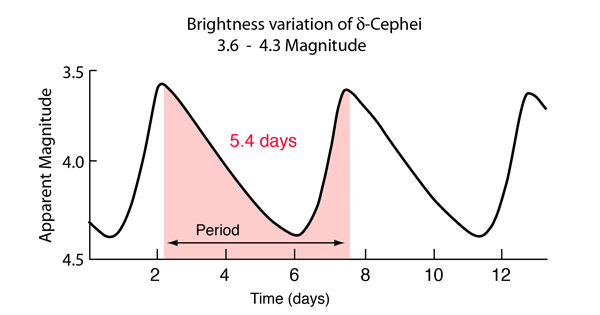
\includegraphics[width=0.5\textwidth]{Images/cephd.png}
    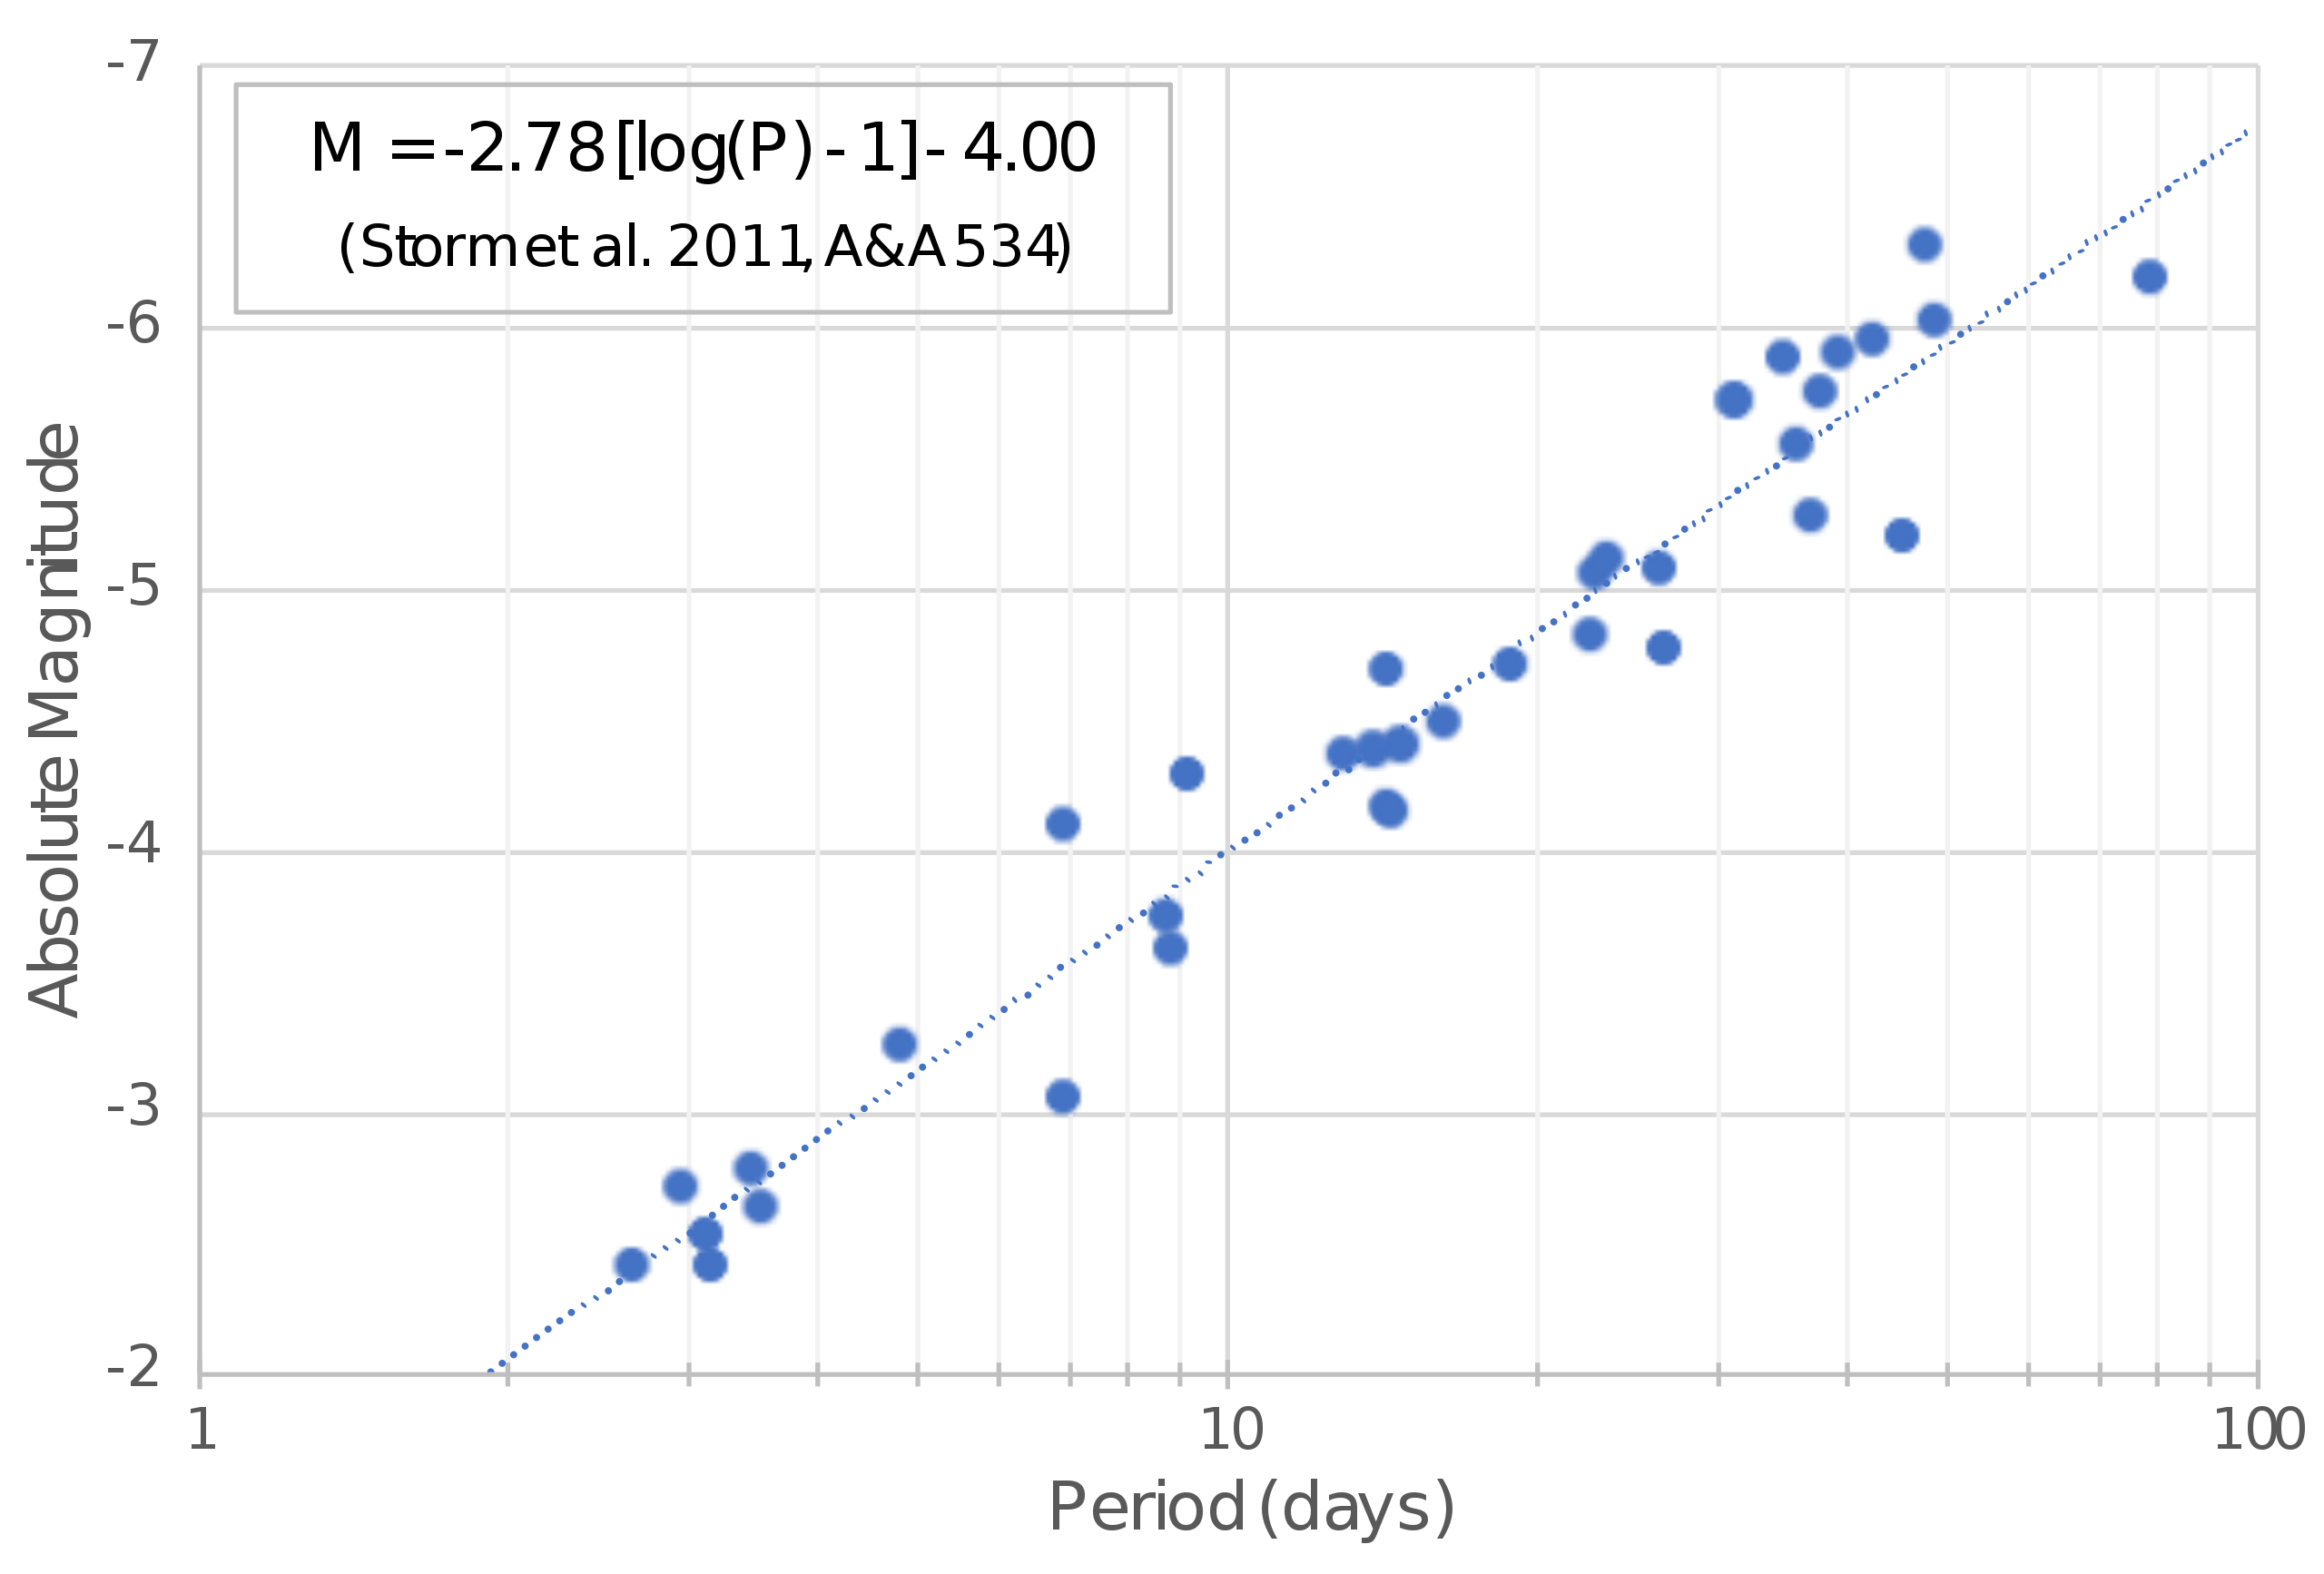
\includegraphics[width=0.40\textwidth]{Images/2560px-Storm2011_Cepheid_Data.svg.png}
    \caption{An illustration of the light curve (measurement of brightness over time) of a Cepheid variable \textsl{(Left)}. The Period-Luminosity relationship for Cepheid variables \textsl{(Right)}.}
    \label{fig:cepheid_periodlum_relationship}
\end{figure}
\medskip \noindent
\textbf{Answer the following questions in your lab notebook}:

\begin{enumerate}
    \item A measured Cepheid has an apparent magnitude of 12 and a pulsation period of 10 days. 
    \begin{enumerate}
        \item Using the period-luminosity relationship given in Figure \ref{fig:cepheid_periodlum_relationship}, determine the absolute magnitude of the Cepheid. (reminder: magnitude measurements don't have units)
        
        \item Use the distance modulus (Equation \ref{eq:dm}) to determine the distance to this Cepheid variable (in parsecs).
        
        \item Recall that a distance in parsecs (measured from the Earth) is related to a parallax angle in arcseconds via $D = 1/\theta$. What is the parallax angle of this Cepheid? Can we measure this parallax using Gaia?
    \end{enumerate} 
    
    \item A different Cepheid has an apparent magnitude of 12 and a pulsation period of 52 days. Determine the distance to this Cepheid variable. 
    
    \item There are a number of steps/measurements involved in finding the distance to a Cepheid variable. What are some sources of error that could cause uncertainty in a Cepheid distance measurement? Recall that Edwin Hubble himself used Cepheid data in his 1929 paper. 
\end{enumerate}

% One way to think about the ``standard candle" method is the following: Imagine you went to the store and bought 10 identical light bulbs. You then went to a dark field and randomly placed the light bulbs at different distances. Since the light bulbs are identical, any difference that you observe in their brightness must be caused by your distance to them (light bulbs further away will seem dimmer). By knowing the inherent brightness of the light bulbs (by measuring its brightness up close), measuring the flux from each of the light bulbs, and using the inverse square law $d^2 = L/4\pi f$ where $d$ is distance, $L$ is luminosity, and $f$ is the measured flux, you can calculate the distance to each of the light bulbs. 

% Henrietta Leavitt found period-luminosity relationship. Maybe show a plot of period and have people find luminosity (which, with a measurement of flux, allows one to compute distance)
\medskip \noindent
While Cepheid variables are useful standard candles, there are also difficulties associated with measuring their distances. One major issue is that Cepheids are simply not bright enough to be measured at cosmological distances. A brighter alternative are \emph{supernovae}.

\subsection{Supernova light curves}
%\textsl{Adapted from \href{http://physics.wm.edu/~labs/astro/}{William and Mary Introductory Astronomy (Physics 177) lab pages}}%

A supernova is the violent explosion of a star. Releasing enormous amounts of energy over the period of a few days, the energy output of a typical supernova can be as much as the total energy output of the Sun \textsl{over its 10 billion-year lifetime}. They are relatively rare events with astronomers estimating that only one or two supernova will occur in the Milky Way every century. While we won't go into detail about supernova classification, they can be broadly classified based on their observed spectra into either Type I (no hydrogen emission lines) or Type II (contains hydrogen emission lines). Supernovae that fall into a subcategory within Type I, called Type Ia (``one-A"), are what are used as standard candles.

\medskip \noindent
Type Ia supernovae, regardless of where they occur in the Universe, are believed to have a fairly consistent peak luminosity since their explosion mechanism is the same. They occur in binary systems (two stars orbiting each other) in which one of the stars is a \textsl{white dwarf}, an extremely dense star with a mass comparable to that of the Sun and a volume comparable to that of Earth. The white dwarf can accrete mass from its companion star until it reaches a critical mass of $1.44\;M_\odot$, beyond which it can no longer support itself against gravitational collapse with electron-degeneracy pressure. Once it exceeds this critical mass, called the \textsl{Chandrasekhar limit}, the carbon in its core will begin fusing and cause the supernova. The consistency in their peak luminosity is due to how white dwarfs are known to explode at the same critical mass. Therefore, Type Ia supernovae are relatively uniform and useful as standard candles.

\medskip \noindent
To get a better understanding of how we can use Type Ia supernovae to obtain cosmological distances, we'll use the ``Supernova Light Curve Fitting Explorer'' contained in the NAAP Labs app. You should already have NAAP Labs downloaded from the Exoplanet Lab; open the app, click on ``14. Cosmic Distance Ladder,'' and select ``Supernova Light Curve Fitting Explorer.'' You should see a plot with magnitude on the vertical axis (absolute magnitude on the left axis and apparent magnitude on the right) and ``Days from Peak'' on the horizontal axis.

\medskip \noindent
The fourth tab of ``hubble.csv'' (the tab labeled ``NAAP SNIa'') lists 6 supernovae. For each of these supernovae, follow these instructions to fill out the spreadsheet.  \textbf{Make sure to include your completed spreadsheet and the appropriate graphs in your lab write-up.}
\begin{enumerate}[label=Step \arabic*:]
    \item At the top right of the NAAP applet screen, select the appropriate supernova from the drop-down menu labeled ``select a supernova.''
    
    \item Check the ``show horizontal bar'’ box.
    
    \item If you click and drag the white area of the plot, you can drag the supernova data points to align with the standard light curve for a Type Ia supernova. The data points can be moved both horizontally and vertically. Align the blue data points with the red template curve.
    
    \item Align the horizontal bar with the peak of the curve. The horizontal bar can be moved by dragging either numerical indicator on the left or right sides of the plot.
    
    \item Input the values of the absolute and apparent magnitudes from the horizontal bar into the ``Distance Modulus Calculator'’ box at the bottom of the applet and read off the value for the distance, $d$, on the bottom right. Record the value of the distance (in Mpc, not pc!) on your spreadsheet.
    
    %\item Calculate the recession velocity of the supernova using the value of the redshift (z) on the spreadsheet and the relationship $v = c \times z$, where $c$ is the speed of light ($c=3.00 \times 10^8\;\mathrm{m/s}$).
\end{enumerate} 

\begin{enumerate}
    \item Once you've fully filled out your spreadsheet, make a scatter plot of your supernova data with the recession velocity on the vertical axis and the distance on the horizontal axis. As you did in Section 2, fit a line to the data to find $H_0$. What value do you get for the Hubble constant?
\end{enumerate}


\section{Conclusions}
\textbf{Answer the following questions in your lab write-up}:
\begin{enumerate}

    \item Qualitatively, what does Hubble's law tell us? What are the physical implications of Hubble's law?
    
    \item What do we mean when we say that the Universe is \emph{expanding}? How does the Hubble constant ($H_0$) relate to the expansion of the Universe?
    
    \item What is the influence of \emph{dark energy} on the expansion of the Universe?

    \item One big problem in modern cosmology (and one of the biggest problems in all of physics) is that \emph{we don't actually know} the correct value of $H_0$ -- measuring the expansion rate of the Universe in two different ways gives us two \emph{completely} different numbers. This problem is called the \textbf{Hubble tension}.
    \begin{enumerate}
        \item Read this short article describing the Hubble tension: \url{https://astrobites.org/2017/10/13/the-hubble-constants/}
        
        \item What are the two primary methods by which astronomers measure $H_0$, and what values of $H_0$ do each of these methods predict?
        
        \item What might we learn by trying to understanding the source of the Hubble tension?
    \end{enumerate}
    
    \item When two neutron stars collide, they release huge amounts of both electromagnetic and gravitational radiation. This radiation -- sometimes referred to as a ``standard siren'' -- can give us both the velocity of and the distance to the host galaxy of the neutron stars, \emph{without} the need for a distance ladder.
    \begin{enumerate}
        \item How can we use standard sirens to measure the Hubble constant?
        
        \item In light of the Hubble tension, why is it useful to have measurements of $H_0$ that don't rely on the distance ladder?
    \end{enumerate}

    \item Write down at least one question that you still have after finishing this lab.
    
    \item If you have any feedback on how today's lab was run, or if you have any suggestions for future lab sessions, please let me know!
    
    
\end{enumerate}


\end{document}